\documentclass{article}
\usepackage[T1]{fontenc}
\usepackage[utf8]{inputenc}
\usepackage{amsmath,amssymb,amsfonts}
\usepackage[english,main=russian]{babel}
\usepackage{graphicx}
\graphicspath{{.}}

\begin{document}

\noindent \textbf{1. Изобразить единичный шар B[0, 1] в пространстве $\langle X, \rho \rangle$}

\textbf{4. $X = \mathbb{R}^3, \rho(x,y) = max\{\lvert x_1 - y_1 \rvert\ + \lvert x_2 - y_2 \rvert, \lvert x_3 - y_3 \rvert\ \}$}

$B[0,1] = \{x \in R^3: \rho(x,0) \leqslant 1 \}$

$\rho(x, 0) =
\begin{cases}
    \lvert x_1 \rvert\ + \lvert x_2 \rvert \text{, если } \lvert x_1 \rvert\ + \lvert x_2 \rvert \geq \lvert x_3\rvert \\
    \lvert x_3 \rvert\ \text{, если } \lvert x_1 \rvert\ + \lvert x_2 \rvert \text{<} \lvert x_3\rvert 
\end{cases}$ 

Рассмотрим $\lvert x_1 \rvert\ + \lvert x_2 \rvert \text{ = } \lvert x_3\rvert$. Проанализируем равенство с помощью фиксации одной из координат. Пусть $x_3$ - константа. Тогда получается равенство $\lvert x_1 \rvert\ + \lvert x_2 \rvert \text{ = c} $ - это ромб, площадь которого увеличивается с увеличением c. Т.к. $\rho \leq 1$, наибольшее значение достигается при $c \in \{-1, 1\}$. Схематические изобразим так:

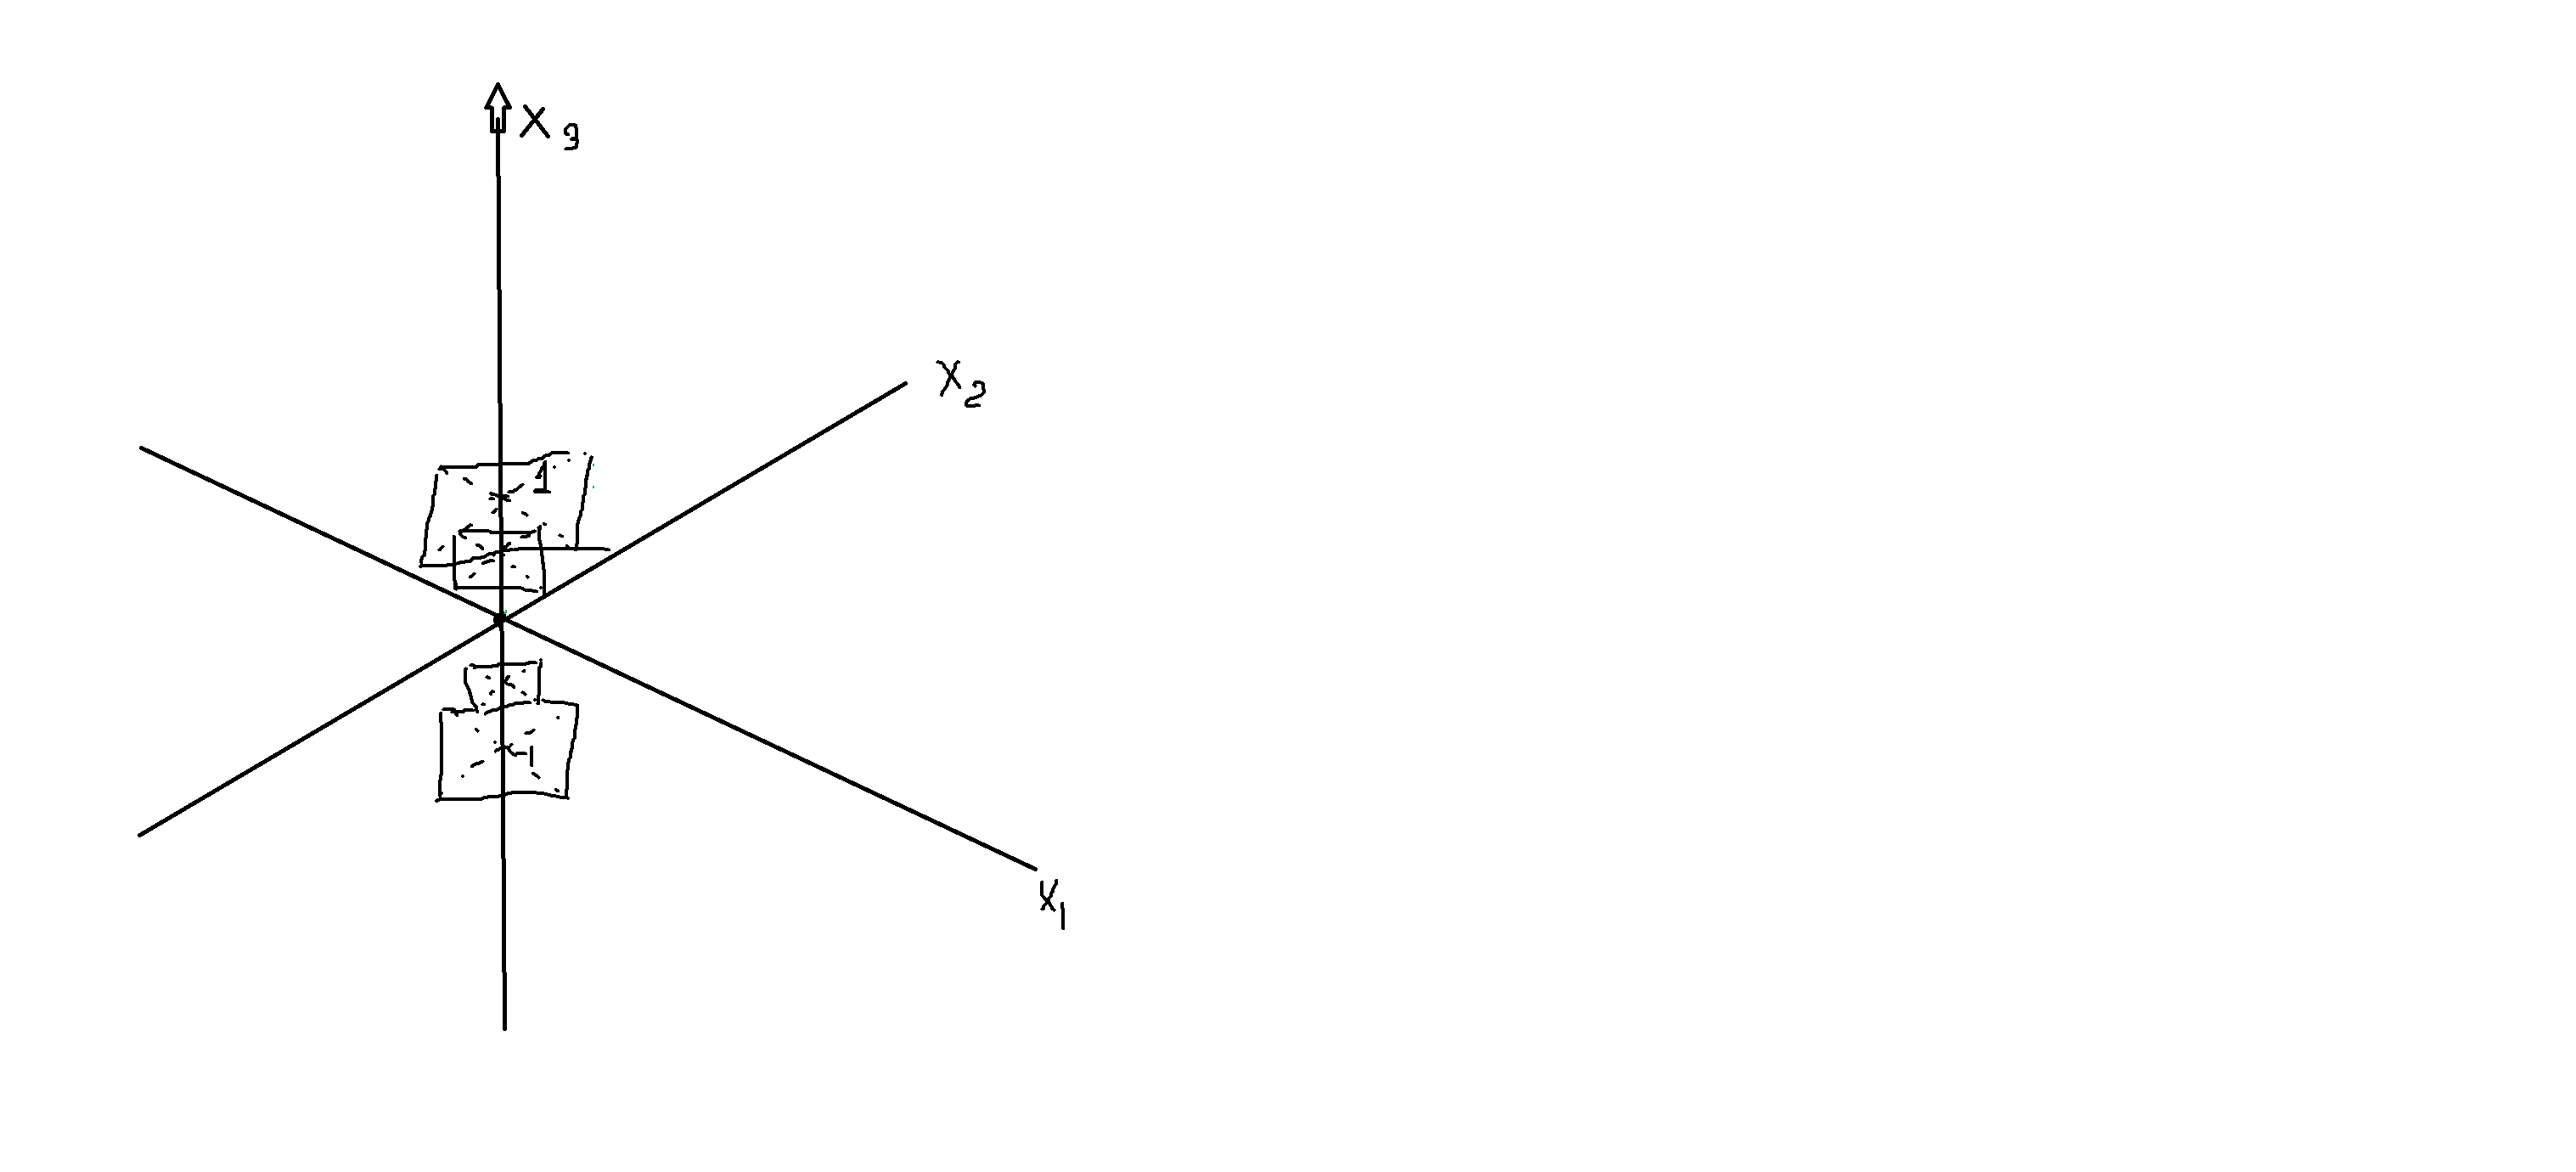
\includegraphics[width=100mm]{Quatreangeold}

Осталось понять, как выглядит объект "сбоку". Для этого зафиксируем другую координату, например, $x_2$, назовем её $k, 1 \geq k \geq 0$. Получается $\lvert x_1 \rvert\ + \text{k} \text{ = } \lvert x_3\rvert$. Это 2 "галки", "вершины" которых перемещаются вдоль оси в зависимости от значения $k$.
Схематические изобразим так:

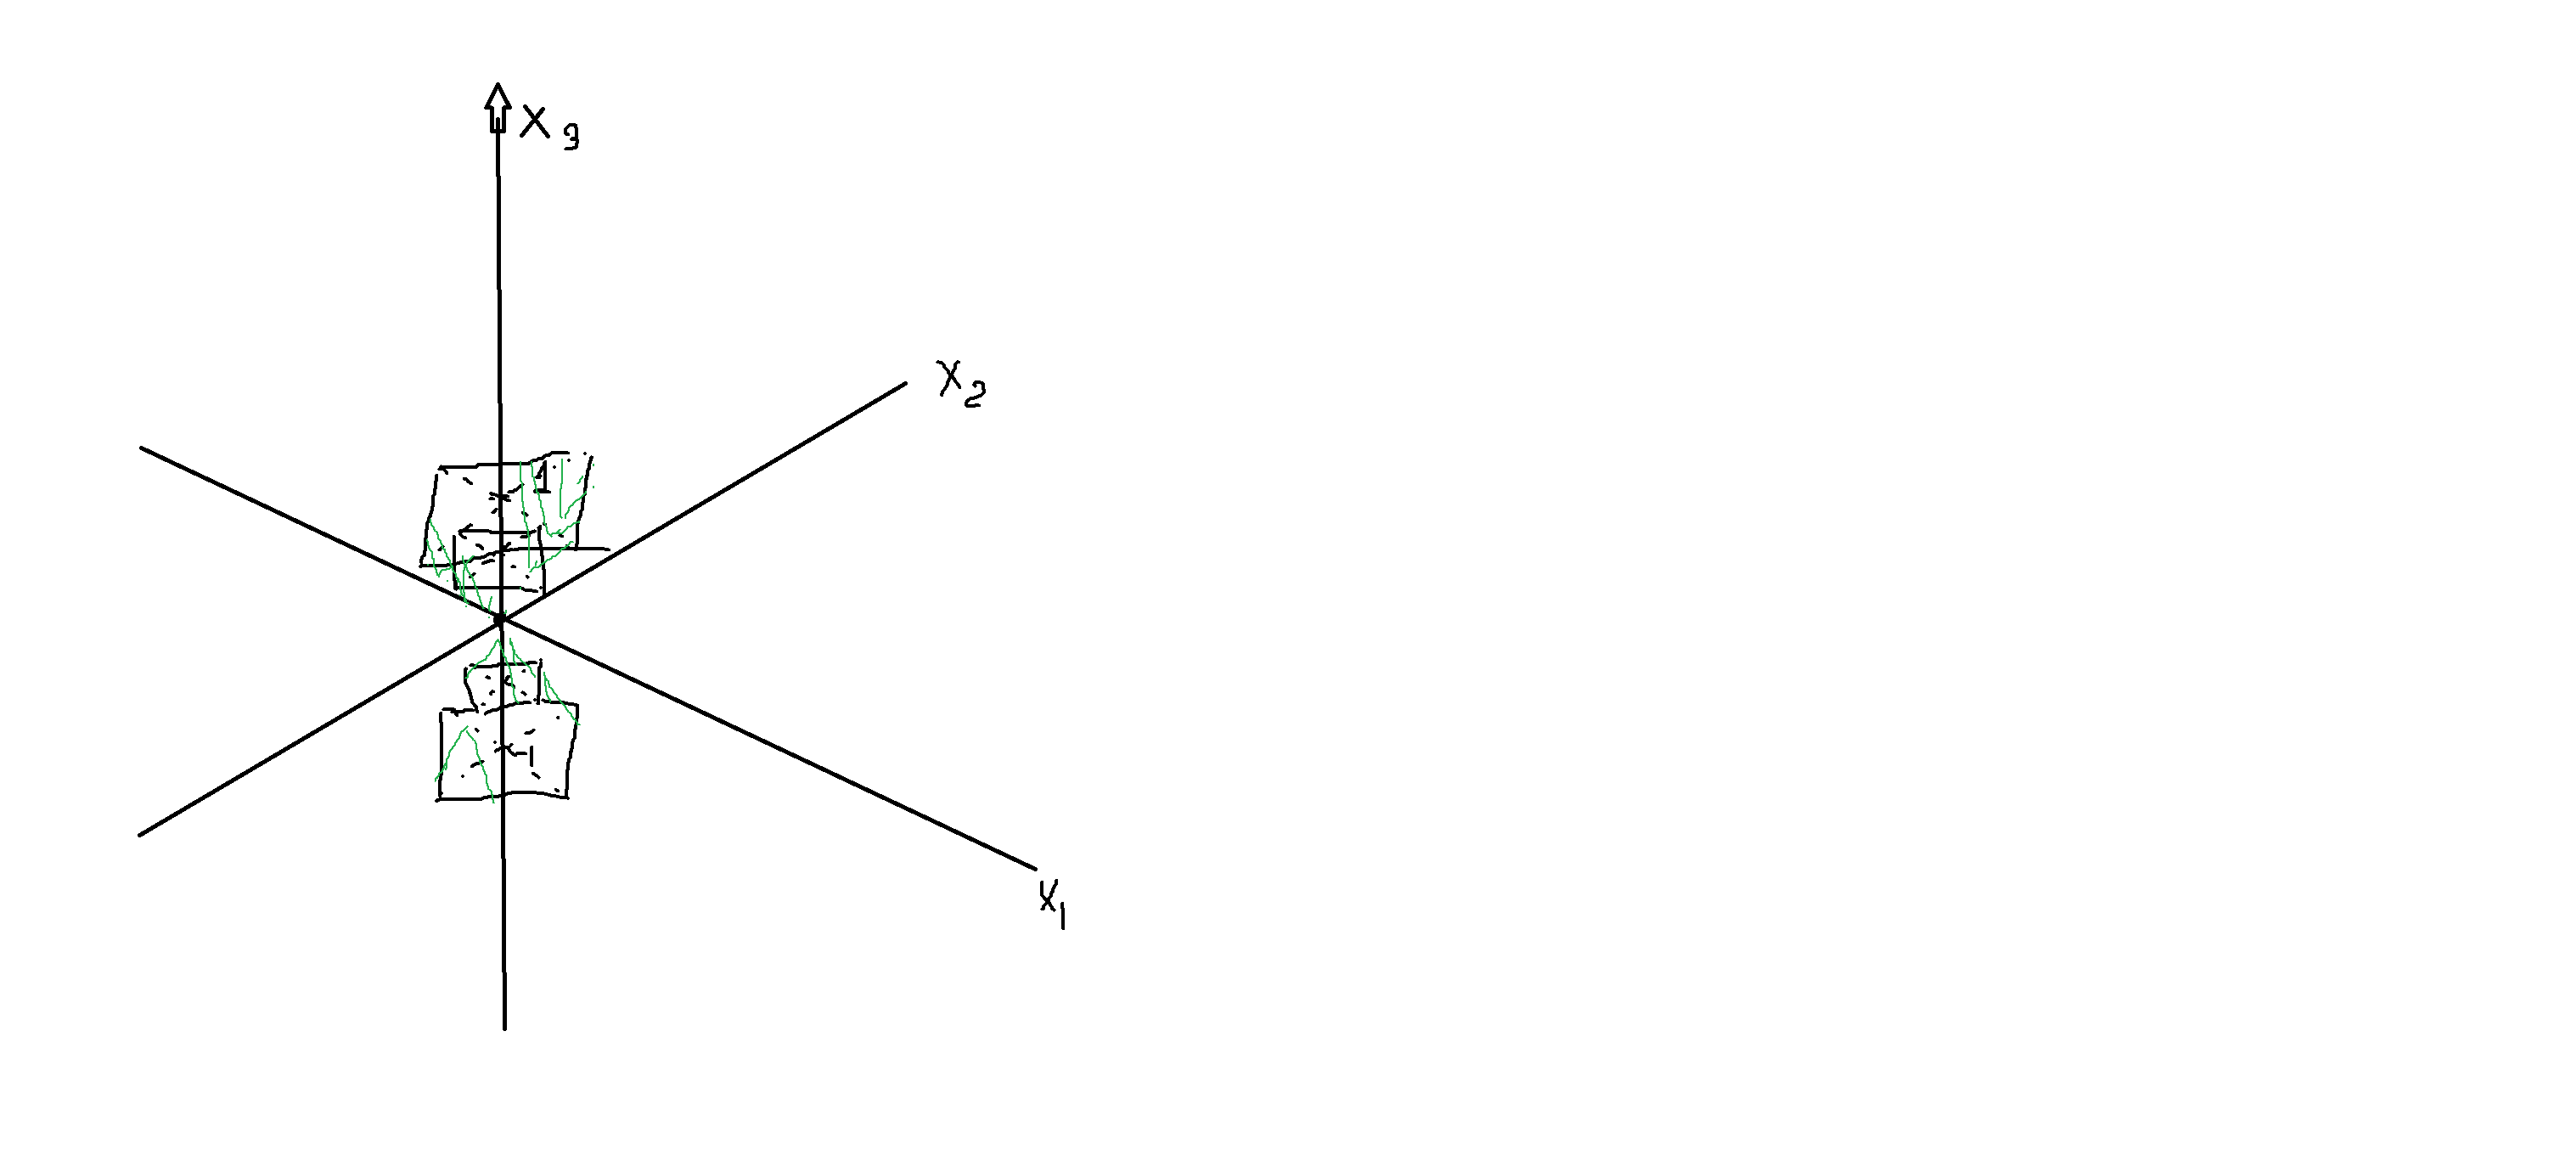
\includegraphics[width=100mm]{Quatreange}

\noindent \textbf{4. Привести примеры метрических пространств, в которых существуют шары}

\textbf{2. совпадающие с множеством своих центров;}

Пусть $X \in \mathbb {N}, r = \frac{1}{2}, \rho(x,y) = \lvert x - y \rvert$, тогда $B[a, r] = \{ x \in \mathbb {N}: \rho(x, a) \leqslant r\}$

Т.к. a $\in \mathbb {N}$, шар будет содержать только натуральные числа - свои центры.

\textbf{3. $B(x_1, r_1)$ и $B(x_2, r_2)$, такие что $B(x_1, r_1) \subset B(x_2, r_2)$, но $r_1 > r_2;$}

Пусть $X \in \mathbb {R},  r_1 = 3, r_2 = 2,  \rho(x,y) =
  \begin{cases}
    \frac{1}{\lvert x - y \rvert} \text{, если } x \neq y\\
    \lvert x + y \rvert \text{, если } x = y 
  \end{cases}$
, тогда $B[2, 3] = \{ x \in \mathbb {R}: \rho(x, 2) \leqslant 3\}$ и $B[1.9, 2] = \{ x \in \mathbb {R}: \rho(x, 1.9) \leqslant 2\}$. 

Эти множества можно изобразить так:


\includegraphics[width=100mm]{Balls}


\textbf{4. $\{B[x_n, r_n]\}^{\infty}_{n=1}, \forall n \in \mathbb {N}: B[x_{n+1}, r_{n+1}] \subset B[x_n, r_n]$, при этом их пересечение пусто $\cap^{\infty}_{n=1} B[x_n, r_n] = \emptyset.$}

Пусть X = (1, 2],  $\rho(x, y) = \lvert x - y \rvert, B[x_n, r_n] = \{x \in X: \rho(x, 1 + \frac{1}{2^n}) \leqslant \frac{1}{2^n}\}$. Очевидно, что $\forall n \in \mathbb {N}: B[x_{n+1}, r_{n+1}] \subset B[x_n, r_n]$, т.к. радиус становится всё меньше и меньше. Если пересечь все такие множества, получится $\emptyset$, потому что при стремлении $n \to \infty$ центр окружности будет стремиться к 1, $x_n \to 1$, что не входит в заданное множество $X$, значит, шар будет состоять только из одного элемента - $\emptyset$. 
\end{document}